
%(BEGIN_QUESTION)
a) En SMART DP-celle er tatt ut av drift og tatt med for benkkalibrering. En automatikker kobler til et presisjons trykkmanometer og en luftkilde til High inngangen på DP-cellen, mens han måler strømutgangen med et multimeter. 

$$\includegraphics[width=15.5cm]{i04815x01.eps}$$

Regn ut avviket i \% av måleområde for {\it sensor trim} og avviket i  \% av måleområde for {\it utgangstrim}.  Forklar hvorfor en må ha en HART kommunikator for å kunne regne disse avvikene sepparat. 


b) Fyll ut kalibreringstabellen for dette strømningsmålesystemet. Systemet består av en måleblende, DP-celle, kvadratrotuttrekker og indikator. Du kan anta følgende måleområder:

Husk:\\
$$Q \propto \sqrt{\Delta P }$$

$$\includegraphics[width=15.5cm]{i00048x01.eps}$$

\begin{itemize}
\item{} FE: 0-50 L/s, 0-100 cmWC  $\Delta$P
\item{} FT: 0-100 cmWC inn, 4-20 mA ut (linear)
\item{} FY: 4-20 mA inn and ut (kvadratrot)
\item{} FI: 4-20 mA inn, 0-50 L/s avlesning
\end{itemize}

% No blank lines allowed between lines of an \halign structure!
% I use comments (%) instead, so that TeX doesn't choke.

$$\vbox{\offinterlineskip
\halign{\strut
\vrule \quad\hfil # \ \hfil & 
\vrule \quad\hfil # \ \hfil & 
\vrule \quad\hfil # \ \hfil & 
\vrule \quad\hfil # \ \hfil & 
\vrule \quad\hfil # \ \hfil & 
\vrule \quad\hfil # \ \hfil \vrule \cr
\noalign{\hrule}
%
% First row
Flow rate & Percent of & Orifice $\Delta$P & FT output & FY output & FI indication \cr
%
% Another row
(L/s) & max. flow (\%) & (cmWC) & signal (mA) & signal (mA) & (L/s) \cr
%
\noalign{\hrule}
%
% Another row
0 & 0 &   &   &   & 0 \cr
%
\noalign{\hrule}
%
% Another row
  & 10 &   &   &   &  \cr
%
\noalign{\hrule}
%
% Another row
  & 25 &   &   &   &  \cr
%
\noalign{\hrule}
%
% Another row
25 & 50 &   &   &   & 25 \cr
%
\noalign{\hrule}
%
% Another row
  & 75 &   &   &   &  \cr
%
\noalign{\hrule}
%
% Another row
  & 90 &   &   &   &  \cr
%
\noalign{\hrule}
%
% Another row
50 & 100 &   &   &   & 50 \cr
%
\noalign{\hrule}
} % End of \halign 
}$$ % End of \vbox

\vfil
%\vfil

%\underbar{file i00000}
%\eject
%(END_QUESTION)





%(BEGIN_ANSWER)


%(END_ANSWER)





%(BEGIN_NOTES)


%INDEX% Alarm, ???: (word or phrase here)
%INDEX% Basics, transmitter: input and output ranges
%INDEX% Basics, ???: (word or phrase here)
%INDEX% Career, ???: (word or phrase here)
%INDEX% Calibration, table: (word or phrase here)
%INDEX% Calibration, ???: (word or phrase here)
%INDEX% Certification exam: (word or phrase here)
%INDEX% Chemistry, ???: (word or phrase here)
%INDEX% Control, proportional: (word or phrase here)
%INDEX% Control, derivative: (word or phrase here)
%INDEX% Control, integral: (word or phrase here)
%INDEX% Control, process characteristics: (word or phrase here)
%INDEX% Control, proportional + derivative: (word or phrase here)
%INDEX% Control, proportional + integral: (word or phrase here)
%INDEX% Control, proportional + integral + derivative: (word or phrase here)
%INDEX% Control, PID tuning: (word or phrase here)
%INDEX% Control, strategies: (word or phrase here)
%INDEX% Control, ???: (word or phrase here)
%INDEX% Course organization, ???: (word or phrase here)
%INDEX% Data Acquisition, ???: (word or phrase here)
%INDEX% DCS, ???: (word or phrase here)
%INDEX% Documentation, P&ID: (word or phrase here)
%INDEX% Documentation, loop diagram: (word or phrase here)
%INDEX% Documentation, functional: (word or phrase here)
%INDEX% Documentation, ???: (word or phrase here)
%INDEX% Electronics review: (word or phrase here)
%INDEX% Fieldbus, ???: (word or phrase here)
%INDEX% Final Control Elements, valve: (word or phrase here)
%INDEX% Final Control Elements, motor: (word or phrase here)
%INDEX% Final Control Elements, pump: (word or phrase here)
%INDEX% Good practices, wiring: ???
%INDEX% Good practices, ???: ???
%INDEX% Lab exercise, ???
%INDEX% Mathematics, calculus: (word or phrase here)
%INDEX% Mathematics, probability: (word or phrase here)
%INDEX% Measurement, pressure: (word or phrase here)
%INDEX% Measurement, level: (word or phrase here)
%INDEX% Measurement, temperature: (word or phrase here)
%INDEX% Measurement, flow: (word or phrase here)
%INDEX% Measurement, analytical: (word or phrase here)
%INDEX% Measurement, ???: (word or phrase here)
%INDEX% Mechanics, pneumatic instrument: (word or phrase here)
%INDEX% Mechanics, ???: (word or phrase here)
%INDEX% Networking, ???: (word or phrase here)
%INDEX% Physics, units and conversions: (word or phrase here)
%INDEX% Physics, energy, work, power: (word or phrase here)
%INDEX% Physics, static fluids: (word or phrase here)
%INDEX% Physics, temperature: (word or phrase here)
%INDEX% Physics, dynamic fluids: (word or phrase here)
%INDEX% Physics, ???: (word or phrase here)
%INDEX% PLC, ???: (word or phrase here)
%INDEX% Relay, ???: (word or phrase here)
%INDEX% Safety, ???: (word or phrase here)
%INDEX% Switch, pressure: (word or phrase here)
%INDEX% Switch, level: (word or phrase here)
%INDEX% Switch, temperature: (word or phrase here)
%INDEX% Switch, flow: (word or phrase here)
%INDEX% Switch, ???: (word or phrase here)
%INDEX% Troubleshooting circuit, ???

%(END_NOTES)


